% !TEX TS-program = pdflatex
% !TEX encoding = UTF-8 Unicode

% This is a simple template for a LaTeX document using the "article" class.
% See "book", "report", "letter" for other types of document.

\documentclass[12pt]{article} % use larger type; default would be 10pt

\usepackage[utf8]{inputenc} % set input encoding (not needed with XeLaTeX)

%%%%\usepackage[document]{ragged2e} 

%%% Examples of Article customizations
% These packages are optional, depending on whether you want the features they provide.
% See the LaTeX Companion or other references for full information.

%%% PAGE DIMENSIONS
\usepackage{geometry} % to change the page dimensions
\geometry{letterpaper} % or letterpaper (US) or a5paper or....
\geometry{margin=1in} % for example, change the margins to 2 inches all round
% \geometry{landscape} % set up the page for landscape
%   read geometry.pdf for detailed page layout information

\usepackage{graphicx} % support the \includegraphics command and options
\graphicspath{
{figs/ipe/}
}
% \usepackage[parfill]{parskip} % Activate to begin paragraphs with an empty line rather than an indent

%%% PACKAGES
\usepackage{booktabs} % for much better looking tables
\usepackage{array} % for better arrays (eg matrices) in maths
\usepackage{paralist} % very flexible & customisable lists (eg. enumerate/itemize, etc.)
\usepackage{epstopdf}
\usepackage{float}
\epstopdfsetup{suffix = {}}
\usepackage{siunitx}
\sisetup{unitsep = \cdot}
\usepackage{verbatim} % adds environment for commenting out blocks of text & for better verbatim
\usepackage{subfig} % make it possible to include more than one captioned figure/table in a single float
% These packages are all incorporated in the memoir class to one degree or another...

\usepackage{caption}        %Allows modification of captions
% \usepackage{indentfirst}    %Allows for indenting first paragraphs



\usepackage{hyperref}
\usepackage{todonotes}

%%% HEADERS & FOOTERS
\usepackage{fancyhdr} % This should be set AFTER setting up the page geometry
\pagestyle{fancy} % options: empty , plain , fancy
\renewcommand{\headrulewidth}{0pt} % customize the layout...
\lhead{}\chead{}\rhead{}
\lfoot{}\cfoot{\thepage}\rfoot{}

%%% SECTION TITLE APPEARANCE
\usepackage{sectsty}
\usepackage{tikz}
\usepackage[framemethod=TikZ]{mdframed}
\usepackage{enumerate}
\usepackage[shortlabels]{enumitem}
\allsectionsfont{\sffamily\mdseries\upshape} % (See the fntguide.pdf for font help)
% (This matches ConTeXt defaults)

%%% ToC (table of contents) APPEARANCE
\usepackage[nottoc,notlof,notlot]{tocbibind} % Put the bibliography in the ToC
\usepackage[titles,subfigure]{tocloft} % Alter the style of the Table of Contents
\renewcommand{\cftsecfont}{\rmfamily\mdseries\upshape}
\renewcommand{\cftsecpagefont}{\rmfamily\mdseries\upshape} % No bold!

%%% END Article customizations

%%% The "real" document content comes below...

\title{Development of an Intelligent Building Energy Management Platform}
\author{Brian Lauer \and Elliot Watkins \and \underline{Advisor}: Dr. Suruz Miah
}
%\date{} % Activate to display a given date or no date (if empty),
         % otherwise the current date is printed 
         
% \setlength{\parindent}{4em} % this should indent paragraphs

\begin{document}
\maketitle


\section{Project Description}
% Significance of the project 
The Internet of Things is a large network of embedded devices like sensors, wearables, and appliances capable of receiving control commands and reporting data over the Internet. Many industries take advantage of this infrastructure to improve process flow and efficiency. One of these industries is the commercial and industrial sector which often employ building automation or management systems to help better manage processes or devices in a building like air conditioning systems, lights or industrial machines. Technological advancements have allowed devices to become connected to a building network through communication protocols like WiFi, Ethernet, Modbus, or BACnet which enables them to be more easily controlled from a central system.
\medbreak\noindent
Our overall goal will be to create a platform in which users can login and access devices connected to a building's energy supply. This allow the user to closely monitor energy usage throughout a commercial or residential building. Additionally, the user will be able to control devices connected to the platform, allowing precise control over the building's energy use.
\medbreak\noindent
The minimum viable product of this project will be to connect to 1 or 2 devices via the the platform and control them. If time allows, we would like to have devices connected to wifi automatically connect to the platform for the user's convenience.

\section{System Architecture}

\subsection{Inputs}
This project will include input from users, smart power meter, devices, and a weather service. Users will be able to adjust the operation of a device (turn up the temperature of an AC unit, for instance) or turn a device on or off completely. Smart power meters will be able to connect the platform and give real-time updates of the building's overall power usage. We would also like to look into meters for individual appliances like AC units and furnaces. The connected devices themselves will continually communicate to the web server their current status. Finally, our platform will regularly receive weather updates from a weather services and warn the user about potential energy loss due to storms.

\subsection{BEMS Core}
A high level view of the operation of the software platform is shown in Figure \ref{fig:functionalBlockDiagram}. Incorporated into the platform will be a web server developed in Python with the Flask web framework. All external and internal HTTP (Hyper Text Transfer Protocol) requests will be processed through this web server in order to store device or user information in the SQLite database. An external request is defined as a request made by a user or device to, for example, update information in the database with a series of SQLite queries. Internal requests are made by other entities or processes running in parallel on the platform including software agents. Similar to BEMOSS, these agents will help to communicate with various devices supported by the platform like broadcasting a discovery service, sending control commands to devices, and regularly requesting data from devices. The platform will be developed and deployed on a Linux machine to encourage support for deployment on SBCs (Single Board Computers) like the Raspberry Pi or BeagleBone Blue to be conveniently stored in a secure location of a building or home like a server cabinet for instance.
\begin{figure}[H]
    \centering
    \includegraphics[scale=0.35]{figs/highLevelArchitecture.pdf}
    \caption{Caption}
    \label{fig:my_label}
\end{figure}
\medbreak\noindent
The SQLite database will be designed to store device information like the device IP address, MAC address, manufacturer name, and device name. A feature will be implemented to allow for customizing the device name. For example, a WeMo Switch connected to the building or home LAN (Local Area Network) could be renamed to "Lamp" or "Light". Secondly, a feature will be added to specify the room or location of each device within the building or home. This will aid any users of the software in distinguishing devices from each other. 
\medbreak\noindent
% Talk about time series feature
Functionality will be avilable in the final version of the platform to store time-series data like on/off status and power data in a database using Apache Cassandra, an open-source NoSQL database management system. This offers a convenient way to log data from device readings in real time. In the future, machine learning algorithms can be used alongside this database to help optimize energy usage.
\medbreak\noindent
A further addition to the software will be added in the form of support for Simscape models, an addon for Simulink to model electromechanical systems. Matlab scripts will be associated with each of these models to collect power data from various electrical models created with Simscape. Using TCP/IP, Matlab will send data from the associated models over the network to the platform to be stored in the Cassandra database.


\begin{figure}[H]
    \centering
    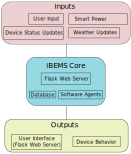
\includegraphics[scale=0.6]{figs/functionalBlockDiagram}
    \caption{High-level Functional Block Diagram}
    \label{fig:functionalBlockDiagram}
\end{figure}
\subsection{Outputs}
The BEMS Core will output all data from devices, smart power meter, and weather updates to the web server. The user will then be able to peruse all available data on any smart device connected to the network.
\section{End-Use Requirements}
By May 2021, users will be able to: remotely turn control devices and monitor energy usage by individual devices.
\medbreak\noindent
Some devices will have more complicated operation than on and off. For example, we plan to add a driver for a beaglebone blue that will include support for the motor drivers. This will require a speed control algorithm capable of precisely regulating motor speed through PWM.
\medbreak\noindent
Since we are writing most of the code in Python, we will use Python's matplotlib module to graph energy usage for a given time period. With the database we plan to implement, we could gather data for a user-defined time period and plot energy usage for that time period. For example, if the user selects a Wemo switch and inputs 10/3/2020 - 10/5/2020, a graph will be generated showing how much energy in kilowatt-hrs that Wemo switch has used.

By May, 2021, we want to have a modular design for the platform that will allow users to add drivers for new devices as they are developed. Once a new device driver is added, the platform will be able to interact with it how the user wants.

\section{Modes of Operation}
To operate properly, the software must include three main modes of operation:
\indent
\begin{enumerate}[leftmargin=*,start=0,label={\bfseries Mode~\#\arabic*:}]
    \item Device discovery mode: the software will be able to discover supported devices automatically upon a device joining the network. To reduce network traffic, the settings page will allow specifying which devices can be discovered.
    \item Manual device control mode: alter the state of devices manually through an easy to use interface in the web UI or through a command line based application accessible through the UI.
    \item Power reporting mode: a page will be available in the UI for reporting the overall power consumption of the building as well as individual device power consumption (if available). 
\end{enumerate}

\end{document}